\section{Connections}

\subsection{Choosing beam and column connections}
The standard method of connecting beams to the web of the colums is to use a rigid connection, for ease of construction. Corner and wind bracings are exempt from this rule, and are mounted directly to the web, as seen in Figure \ref{fig:cornerBracing}.


\begin{figure}[H]
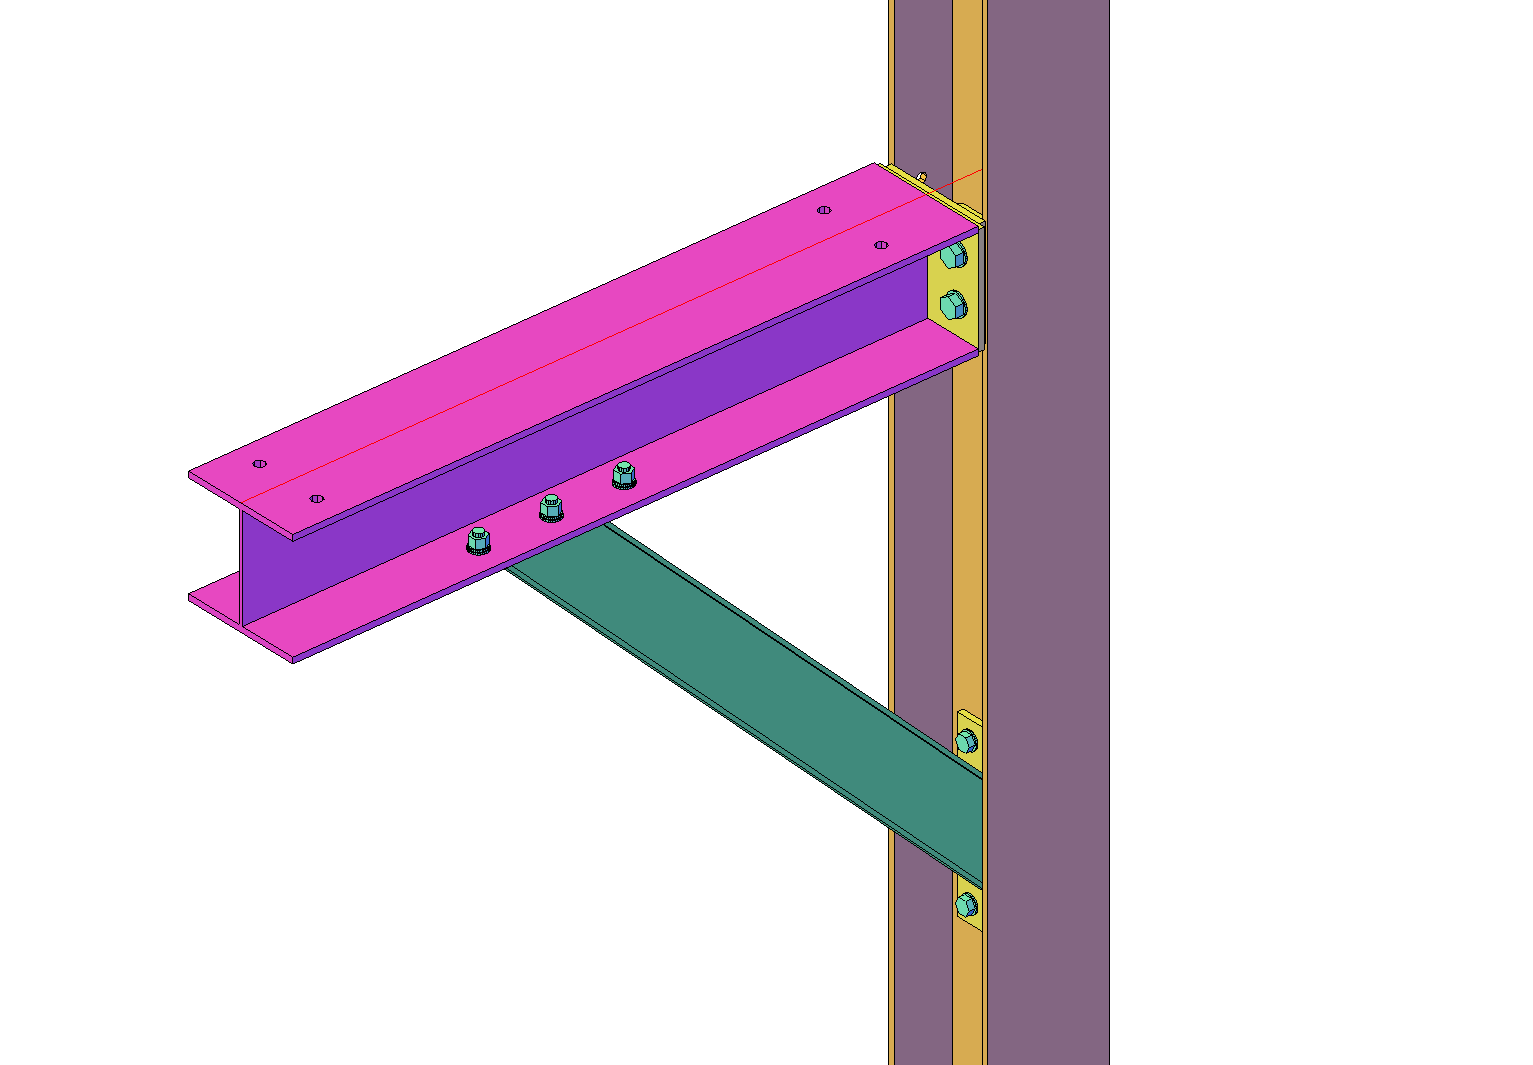
\includegraphics[width=.8\textwidth]{cornerBracing}
\caption{A standard beam and corner bracing connected to a column}\label{fig:cornerBracing}
\end{figure}

\subsection{Mounting conveyors and machines}
Whenever possible UNP and angle is used to mount the conveyors and machines. Folded plate is used when the other options are deemed not possible or practical.\\
Mounting profiles on conveyors and other options have to be present in the sales models, to avoid any mistakes or misconceptions.\\